\chapter{Experimental Results}

The system is tested against a library database. The system gives satisfactory results for both simple queries and complex queries with foreign key-primary key relationships along with aggregate functions. As the implementation only incorporates single word attributes, testing it for complex database is difficult. A syntactically correct SQL query is almost always generated for a correctly mapped parse tree. The figure \ref{fig:schema} represents the schema for the library database,\\

\begin{figure}[htb]
\centering
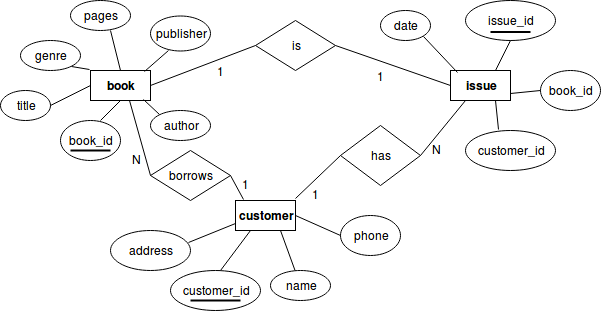
\includegraphics[scale=0.55]{./er} % e.g. insert ./image for image.png in the working directory, adjust scale as necessary
\caption{Schema for library database}
\label{fig:schema} % insert suitable label, this is used to refer to a fig from within the text as shown above
\end{figure}




\section{Simple queries}

\begin{enumerate}
\item \textbf{Input: Give me every book.}\\
\textbf{Query:}\\SELECT book FROM book;\\
\textbf{Output:}\\
('(1,Heartless,Stephens,Romantic,123,Martin)',)\\
('(2,King,Khan,Action,342,Khan)',)\\
('(3,Lord,Bose,History,233,BPB)',)\\
...\\
('(25,Beautiful,Oldman,Romantic,389,McGrawHill)',)\\
('(26,Mind,Narayana,Science,612,Scifi)',)\\
('(27,Tempest,Narayana,Science,231,Scifi)',).


\item \textbf{Return all book titles and pages.}\\
\textbf{Query:}\\SELECT book.title, book.pages FROM book;\\
\textbf{Output:}\\
('Heartless', 123), ('King', 342), ('Lord', 233),\\
......,\\
,('Beautiful', 389),('Mind', 612),('Tempest', 231).

\item \textbf{
Fetch all customer name and address.}\\
\textbf{Query:}\\SELECT customer.name, customer.address FROM customer;\\
\textbf{Output:}\\
('John', 'Delhi'),('Adam', 'Delhi'),('Kishor', 'Mumbai')\\
...\\
('Suraj', 'Delhi'),('Chaitanya', 'Raigarh'),('Neeraj', 'Raipur').

\item \textbf{Fetch all book whose author is Amrish.}\\
\textbf{Query:}\\SELECT book FROM book WHERE book.author = 'Amrish';\\
\textbf{Output:}\\
('(21,Shiva,Amrish,Drama,543,Tripathi)',),\\
('(22,Shiva2,Amrish,Drama,323,Tripathi)',),\\
('(23,Shiva3,Amrish,Drama,464,Tripathi)',).

\item \textbf{Return name of customers who are not living in Mumbai.}\\
\textbf{Query:}\\
SELECT customer.name FROM customer\\
WHERE customer.address != 'Mumbai';\\
\textbf{Output:}\\
('John',),('Adam',),('Kamlesh',),('Akshay',),('Jobin',),('Nirant',),\\
('Anurag',),('Bhupendra',),('Harshit',),('Balmukund',),('Vipin',),('Mayank',)\\
('Anand',),('Astik',),('Ashok',),('Prabhav',),('Suraj',),('Chaitanya',),('Neeraj',)\\

\item \textbf{Return count of customer we have.}\\
\textbf{Query:}\\SELECT COUNT(customer) FROM customer;\\
\textbf{Output:}\\ (22)

\item \textbf{Return number of books.}\\
\textbf{Query:}\\SELECT COUNT(book) FROM book;\\
\textbf{Output:}\\ (27)

\item \textbf{Return average pages in books.}\\
\textbf{Query:}\\SELECT AVG(book.pages) FROM book;\\
\textbf{Output:}\\ ('424.0370370370370370')

\end{enumerate}

\section{Complex queries}

\begin{enumerate}
\item \textbf{Return name of customer who issued a book named Inception.}\\
\textbf{Query:}\\SELECT issue, customer.name\\
FROM customer, book, issue\\
WHERE book.book\_id = issue.book\_id\\ 
AND customer.customer\_id = issue.customer\_id\\ 
AND book.title = 'Inception' \\
AND issue.book\_id = book.book\_id;\\
\textbf{Output:}\\ ('(16,19,12,2009)', 'Vishal')

\item \textbf{Print all book published by Tripathi publications and whose genre is Drama.}\\
\textbf{Query:}\\SELECT book FROM book \\
WHERE book.genre = 'Drama' AND book.publisher = 'Tripathi';\\
\textbf{Output:}\\
('(21,Shiva,Amrish,Drama,543,Tripathi)',),\\
('(22,Shiva2,Amrish,Drama,323,Tripathi)',),\\
('(23,Shiva3,Amrish,Drama,464,Tripathi)',)

\item \textbf{fetch all customers names  who issued Drama book of Amrish.}\\
\textbf{Query:}\\SELECT issue, customer.name \\
FROM customer, book, issue\\
WHERE book.genre = 'Drama' AND book.book\_id = issue.book\_id \\
AND customer.customer\_id = issue.customer\_id \\
AND book.author = 'Amrish' \\
AND issue.book\_id = book.book\_id;\\
\textbf{Output:}\\
('(17,21,13,2011)', 'Vipin')\\
('(18,22,14,2015)', 'Mayank')\\
('(19,23,14,2013)', 'Mayank')\\

\item \textbf{fetch all customers names  who have not issued any book of Amrish.}\\
\textbf{Query:}\\SELECT customer.name, issue\\
FROM customer, book, issue\\
WHERE book.book\_id = issue.book\_id\\
AND customer.customer\_id = issue.customer\_id\\
AND book.author != 'Amrish'\\ 
AND issue.book\_id = book.book\_id;\\
('John', '(1,1,0,2015)'),('Adam', '(2,2,1,2016)'),('Adam', '(3,3,1,2015)')\\
....\\
('Bhupendra', '(14,16,9,2011)'),('Anurag', '(15,17,8,2010)'),('Vishal', '(16,19,12,2009)')\\

\item \textbf{fetch all customer who have issued any book before 2014.}\\
\textbf{Query:}\\SELECT customer\\
FROM customer, issue\\
WHERE customer.customer\_id = issue.customer\_id \\
AND issue.date < 2014;\\
\textbf{Output:}\\
('(2,Kishor,Mumbai,9147542363)',),('(3,Kamlesh,Raigarh,9148954662)',),\\
('(3,Kamlesh,Raigarh,9148954662)',),('(5,Jobin,Calicut,9147242426)',),\\
('(5,Jobin,Calicut,9147242426)',),('(8,Anurag,Raigarh,7332842921)',),\\
('(8,Anurag,Raigarh,7332842921)',),('(9,Bhupendra,Raipur,7332821414)',),\\
('(12,Vishal,Mumbai,7332842921)',),('(13,Vipin,Calicut,7332842923)',),\\
('(14,Mayank,Bilaspur,8522424413)',)

\item \textbf{Return customer name , address and issue date of book Shiva.}\\
\textbf{Query:}\\SELECT issue.date, customer.address, customer.name\\
FROM customer, book, issue\\
WHERE book.book\_id = issue.book\_id\\
AND customer.customer\_id = issue.customer\_id\\
AND book.title = 'Shiva'\\
AND issue.book\_id = book.book\_id;\\
\textbf{Output:}\\
(2011, 'Calicut', 'Vipin')

\item \textbf{Return count of customer we have who issued book before 2016.}\\
\textbf{Query:}\\SELECT COUNT(customer)\\
FROM customer, issue\\
WHERE customer.customer\_id = issue.customer\_id\\
AND issue.date < 2016;\\
Output: \\
(18)

\item \textbf{Return average pages in books by Amrish.}\\
\textbf{Query:}\\SELECT AVG(book.pages)\\
FROM book\\
WHERE book.author = 'Amrish';\\
\textbf{Output:}\\
('443.3333333333333333')\\


\item \textbf{print the number of customer do we have whose name is Anurag?}\\
\textbf{Query:}\\SELECT COUNT(customer)\\
FROM customer\\
WHERE customer.name = 'Anurag';\\
\textbf{Output:}\\
(1)

\item \textbf{Return name and phone of customer who lives in Delhi.}\\
\textbf{Query:}\\SELECT customer.phone, customer.name\\
FROM customer\\
WHERE customer.address = 'Delhi';\\
\textbf{Output:}\\
('9567843232', 'John')\\
('9547543332', 'Adam')\\
('73328423231', 'Harshit')\\
('7332323923', 'Astik')\\
('7332842867', 'Suraj')\\


\end{enumerate}


We tested the system on a total of 47 queries. The following is the tabulated results.

\begin{figure}[htb]
\centering
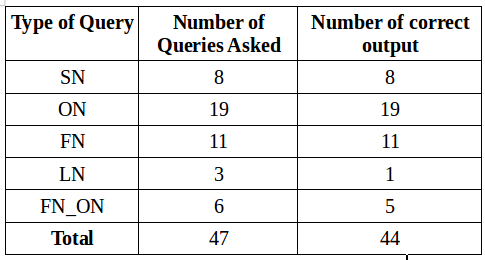
\includegraphics[scale=0.55]{./Results} % e.g. insert ./image for image.png in the working directory, adjust scale as necessary
\caption{Results}
\label{fig:grammar} % insert suitable label, this is used to refer to a fig from within the text as shown above
\end{figure}

\begin{itemize}
    \item SN : simple queries in which the query tree only has SN,NN,VN nodes
    \item ON : queries having SN,NN,VN and ON nodes  
    \item {FN : queries having SN,NN,VN and FN nodes  }
    \item {LN : queries having SN,NN,VN and LN nodes  }
    \item {FN\_ON : queries having SN,NN,VN,FN and ON nodes  }
\end{itemize}
    
    



